\section{Algorithm}
\begin{frame}{Simplifying the Model -- Reachability Game with Nature}
\begin{columns}
\column{.5\textwidth}
\vspace{5mm}
\only<-2>{
\begin{tikzpicture}[>=stealth, node distance=3cm, every node/.style={font=\small}]

% Nodes
\node[draw, minimum size=1cm, shape=rectangle] (S1) {$s_1$};
\node[draw, minimum size=1cm, shape=circle,right= 5cm of S1] (S2) {$s_2$};
\node[draw, minimum size=1cm, shape=circle, below= 3cm of $(S1)!0.5!(S2)$] (S3) {$s_3$};

\draw[-] (S1) -- node[below left, pos=0.5] {$a$} ($(S1)!0.5!(S3)$);
\filldraw[black] ($(S1)!0.5!(S3)$) circle (2pt); % Dot at split point
\draw[->] ($(S1)!0.5!(S3)$) -- node[below left, pos=0.5] {$\frac{2}{3}$} (S3);
\draw[->] ($(S1)!0.5!(S3)$) -> node[below, pos=0.75] {$\frac{1}{3}$} (S2);
\draw[-] (S2) -- node[below right, pos=0.5] {$a$} ($(S2)!0.5!(S3)$);
\filldraw[black] ($(S2)!0.5!(S3)$) circle (2pt); % Dot at split point
\draw[->] ($(S2)!0.5!(S3)$) -- node[below right, pos=0.5] {$\frac{1}{2}$} (S3);
\draw[->] ($(S2)!0.5!(S3)$) -- node[below, pos=0.75] {$\frac{1}{2}$} (S1);

\draw[->] (S1) to[bend left=30] node[above, pos=0.25] {$b$} 
node[above, pos=0.75] {$1$} coordinate[pos=0.5] (S1S2) (S2);
\filldraw[black] (S1S2) circle (2pt); % Dot halfway along the curve

\draw[->] (S2) -> node[above, pos=0.25] {$b$} node[above, pos=0.75] {$1$} coordinate[pos=0.5] (S2S1) (S1);
\filldraw[black] (S2S1) circle (2pt); % Dot halfway along the curve

\draw[->] (S3) edge[loop below]
coordinate[pos=0.5] (S3S3)
node[right, pos=0.2] {$c$}
node[left, pos=0.8] {$1$} (S3);
\filldraw[black] (S3S3) circle (2pt); % Dot halfway along the curve

\end{tikzpicture}
}
\only<3->{
\begin{tikzpicture}[>=stealth, node distance=3cm, every node/.style={font=\small}]
% Nodes
\node[draw, minimum size=1cm, shape=rectangle] (S1) {$s_1$};
\node[draw, minimum size=1cm, shape=circle,right= 5cm of S1] (S2) {$s_2$};
\node[draw, minimum size=1cm, shape=circle, below= 3cm of $(S1)!0.5!(S2)$] (S3) {$s_3$};
\draw[-] (S1) -- node[below left, pos=0.5] {} ($(S1)!0.5!(S3)$);
\filldraw[black] ($(S1)!0.5!(S3)$) circle (2pt) 
    node[label={225:$(s_1,a)$}] {}; % Labeled dot at split point
    
\draw[->] ($(S1)!0.5!(S3)$) -- node[below left, pos=0.5] {} (S3);
\draw[->] ($(S1)!0.5!(S3)$) -> node[below, pos=0.75] {} (S2);
\draw[-] (S2) -- node[below right, pos=0.5] {} ($(S2)!0.5!(S3)$);
\filldraw[black] ($(S2)!0.5!(S3)$) circle (2pt) 
    node[label={315:$(s_2,a)$}] {}; % Labeled dot at split point
    
\draw[->] ($(S2)!0.5!(S3)$) -- node[below right, pos=0.5] {} (S3);
\draw[->] ($(S2)!0.5!(S3)$) -- node[below, pos=0.75] {} (S1);
\draw[->] (S1) to[bend left=30] node[above, pos=0.25] {} 
node[above, pos=0.75] {} coordinate[pos=0.5] (S1S2) (S2);
\filldraw[black] (S1S2) circle (2pt) 
    node[label={90:$(s_1, b)$}] {}; % Labeled dot halfway along the curve
    
\draw[->] (S2) -> node[above, pos=0.25] {} node[above, pos=0.75] {} coordinate[pos=0.5] (S2S1) (S1);
\filldraw[black] (S2S1) circle (2pt) 
    node[label={270:$(s_2, b)$}] {}; % Labeled dot halfway along the curve
    
\draw[->] (S3) edge[loop below]
coordinate[pos=0.5] (S3S3)
node[right, pos=0.2] {}
node[left, pos=0.8] {} (S3);
\filldraw[black] (S3S3) circle (2pt) 
    node[label=270:{$(s_3, c)$}] {}; % Labeled dot halfway along the curve
    
\end{tikzpicture}
}
\column{.5\textwidth}
\begin{itemize}[<+->]
    \item Remove precise probabilities
    \item Probabilistic decisions become\\
    \alert{nature states}
    \item Result: RGN $\mathcal{P}=(S_0, S_1, S_N, E)$
    \item Ordinary \alert{labeled directed graph}
\end{itemize}
\uncover<+->{
\vspace{5mm}
\hspace{-5mm}In this case: $S_0=\set{s_1, s_3}$, $S_1=\set{s_2}$,\\
\hspace{-5mm}$S_N=\set{(s_1, a), (s_1, b), (s_2, a), (s_2, b), (s_3, c)}$
}
\end{columns}
\end{frame}
\iffalse
\begin{frame}{Strong Attractors -- Computing $\Reach_i(T, \mathcal{G})$}
\begin{columns}
\column{0.5\textwidth}
    \uncover<+->{
    We build up a working set $A_k$:
    }
    \begin{itemize}[<+->]
        \item Start off with the target set $T$
        \item We can add a state $s$ leading to the working set if:
        \begin{itemize}[<+->]
            \item It belongs to player $i$.
            \item It's a nature state.
            \item It belongs to player $1-i$ and all it's successors are in the working set.
        \end{itemize}
    \end{itemize}
\column{0.5\textwidth}
    \begin{alignat*}{3}
        \uncover<2->{A_0 &\defeq T}\\
        \uncover<4->{A_{k+1} &\defeq A_k&&\cup\{s\in &&\Pred(A_k): s\in S_i\}}\\
        \uncover<5->{        &          &&\cup\{s\in &&\Pred(A_k): s\in S_N\}}\\
        \uncover<6->{        &          &&\cup\{s\in &&\Pred(A_k): s\in S_{1-i}}\\
        \uncover<6->{        &          &&           &&\text{ and } \Succ(s)\subseteq A_k\}}\\
    \end{alignat*} 
    \vspace{-1cm}
        \uncover<7->{\[
        \satr(T, \mathcal{P}) \defeq \bigcup_{k\in\N} A_k\]}
\end{columns}
    
\end{frame}
\fi

\begin{frame}{Strong Attractors -- Computing $\Reach_i(T, \mathcal{G})$}
    \uncover<1->{We build up a working set $A_k$}:
    \begin{alignat*}{4}
        \uncover<2->{A_0 &\defeq T}     &&           &&                                      &&\uncover<3->{T\subseteq\Reach_i(T,\mathcal{G})}\\
        \uncover<4->{A_{k+1} &\defeq A_k&&\cup\{s\in &&\Pred(A_k): s\in S_i\}}               &&\uncover<5->{s\text{ belongs to player }i}\\
        \uncover<6->{        &          &&\cup\{s\in &&\Pred(A_k): s\in S_N\}}               &&\uncover<7->{s\text{ belongs to the nature player}}\\
        \uncover<8->{        &          &&\cup\{s\in &&\Pred(A_k): s\in S_{1-i}}             &&\uncover<9->{s\text{ belongs to the player } 1-i \text{ and}}\\
        \uncover<8->{        &          &&           &&\text{ and } \Succ(s)\subseteq A_k\}} \hspace{8mm}&&\uncover<9->{\text{all successors are in } A_k}\\
    \end{alignat*} 
        \vspace{-1.5cm}
        
        \uncover<10->{\[\satr(T, \mathcal{P}) \defeq \bigcup_{k\in\N} A_k\]}
    
\end{frame}

\begin{frame}{Strong Attractors -- Example\hfill $\satr_0(T=\set{s_3}, \mathcal{P})$}
\begin{columns}
\column{0.4\textwidth}
\vspace{5mm}

\begin{tikzpicture}[>=stealth, node distance=3cm, every node/.style={font=\small}]
% Nodes
\node[draw, minimum size=1cm, shape=rectangle] (S1) {$\textcolor<4->{myblue}{\textcolor<3>{orange}{s_1}}$};
\node[draw, minimum size=1cm, shape=circle,right= 5cm of S1] (S2) {$\textcolor<5->{myblue}{\textcolor<5>{orange}{s_2}}$};
\node[draw, minimum size=1cm, shape=circle, below= 3cm of $(S1)!0.5!(S2)$] (S3) {$\textcolor<2->{myblue}{\textcolor<1>{orange}{s_3}}$};
\draw[-] (S1) -- node[below left, pos=0.5] {} ($(S1)!0.5!(S3)$);
\filldraw[black] ($(S1)!0.5!(S3)$) circle (2pt) 
    node[label={225:$\textcolor<3->{myblue}{\textcolor<2>{orange}{(s_1,a)}}$}] {}; % Labeled dot at split point
    
\draw[->] ($(S1)!0.5!(S3)$) -- node[below left, pos=0.5] {} (S3);
\draw[->] ($(S1)!0.5!(S3)$) -> node[below, pos=0.75] {} (S2);
\draw[-] (S2) -- node[below right, pos=0.5] {} ($(S2)!0.5!(S3)$);
\filldraw[black] ($(S2)!0.5!(S3)$) circle (2pt) 
    node[label={315:$\textcolor<3->{myblue}{\textcolor<2>{orange}{(s_2,a)}}$}] {}; % Labeled dot at split point
    
\draw[->] ($(S2)!0.5!(S3)$) -- node[below right, pos=0.5] {} (S3);
\draw[->] ($(S2)!0.5!(S3)$) -- node[below, pos=0.75] {} (S1);
\draw[->] (S1) to[bend left=30] node[above, pos=0.25] {} 
node[above, pos=0.75] {} coordinate[pos=0.5] (S1S2) (S2);
\filldraw[black] (S1S2) circle (2pt) 
    node[label={90:$\textcolor<7->{myblue}{\textcolor<6>{orange}{(s_1, b)}}$}] {}; % Labeled dot halfway along the curve
    
\draw[->] (S2) -> node[above, pos=0.25] {} node[above, pos=0.75] {} coordinate[pos=0.5] (S2S1) (S1);
\filldraw[black] (S2S1) circle (2pt) 
    node[label={270:$\textcolor<5->{myblue}{\textcolor<4>{orange}{(s_2, b)}}$}] {}; % Labeled dot halfway along the curve
    
\draw[->] (S3) edge[loop below]
coordinate[pos=0.5] (S3S3)
node[right, pos=0.2] {}
node[left, pos=0.8] {} (S3);
\filldraw[black] (S3S3) circle (2pt) 
    node[label=270:{$\textcolor<3->{myblue}{\textcolor<2>{orange}{(s_3, c)}}$}] {}; % Labeled dot halfway along the curve
    
\end{tikzpicture}

\column{0.6\textwidth}
\small
\hspace{-2mm}
\begin{align*}
    \uncover<+->{A_0 &=\set{\textcolor<1>{orange}{s_3}}}\\
    \uncover<+->{A_1 &=\set{\textcolor<2>{myblue}{s_3,} \textcolor<2>{orange}{(s_1, a), (s_2, a), (s_3, c)}}}\\
    \uncover<+->{A_2 &=\set{\textcolor<3>{myblue}{s_3, (s_1, a), (s_2, a), (s_3, c),} \textcolor<3>{orange}{s_1}}}\\
    \uncover<+->{A_3 &=\set{\textcolor<4>{myblue}{s_3, (s_1, a), (s_2, a), (s_3, c), s_1,} \textcolor<4>{orange}{(s_2, b)}}}\\
    \uncover<+->{A_4 &=\set{\textcolor<5>{myblue}{s_3, (s_1, a), (s_2, a), (s_3, c), s_1, (s_2, b),} \textcolor<5>{orange}{s_2}}}\\
    \uncover<+->{A_5 &=\set{\textcolor<6->{myblue}{s_3, (s_1, a), (s_2, a), (s_3, c), s_1, (s_2, b), s_2,} \textcolor<6->{orange}{(s_1, b)}}}\\
    \uncover<+->{A_k &=A_5\quad\text{for }k\geq 5}\\
    \uncover<+->{\satr_0(\set{s_3}, \mathcal{P})&=\set{s_3, (s_1, a), (s_2, c), (s_3, c), s_1, (s_2, b), s_2, (s_1, b)}}
\end{align*}
    
\end{columns}
\end{frame}
\begin{frame}{Strong Attractors Compute Positive Reachability}
Let $\mathcal{G}$ be an SMG and $\mathcal{P}$ the corresponding RGN, $i\in\set{0,1}$. It holds that:
\vspace{1cm}

\LARGE
\[
        \satr_i(T, \mathcal{P})\cap S = \Reach_i(T, \mathcal{G})
\]
\normalsize
\vspace{1cm}

Proof in thesis.
\end{frame}

\begin{frame}{Weak Attractors -- Computing $\ASReach_i(T, \mathcal{G})$}
\vfill

\uncover<+->{We shrink a working set $B_k$:}
\begin{alignat*}{2}
\uncover<+->{B_0 &\defeq\satr_i(T, \mathcal{P})                                        }&&\uncover<+->{\ASReach_i(T,\mathcal{G})\subseteq \Reach_i(T,\mathcal{G})}\\
\uncover<+->{C_k &\defeq\satr_{1-i}(S\setminus B_k, \mathcal{P}\setminus T)\hspace{6mm}}&&\uncover<+->{\text{States from which player $i-1$ can enforce leaving $B_k$}}\\
\uncover<+->{B_{k+1} &\defeq\satr_i(T, \mathcal{P}\setminus C_k)                       }&&\uncover<+->{\text{Remove $C_k$ from the graph}}\\
\end{alignat*}
\uncover<+->{
\vspace{-0.7cm}
\[
\watr_i(T,\mathcal{P}) =\bigcap_{k\in\N}B_k
\]
}
\vfill
\end{frame}

\begin{frame}{Weak Attractors -- Computing $\ASReach_i(T, \mathcal{G})$}
\begin{columns}
\column{0.5\textwidth}
        \centering
\hfill\begin{align*}
B_0 &\defeq\satr_i(T, \mathcal{P})\\
C_k &\defeq\satr_{1-i}(S\setminus B_k, \mathcal{P}\setminus T)\\
B_{k+1} &\defeq\satr_i(T, \mathcal{P}\setminus C_k)\\
\end{align*}
\[
\watr_i(T,\mathcal{P}) =\bigcap_{k\in\N}B_k
\]
\column{0.5\textwidth}
        \centering
        \vspace{-3.5mm}

        \hspace{-1cm}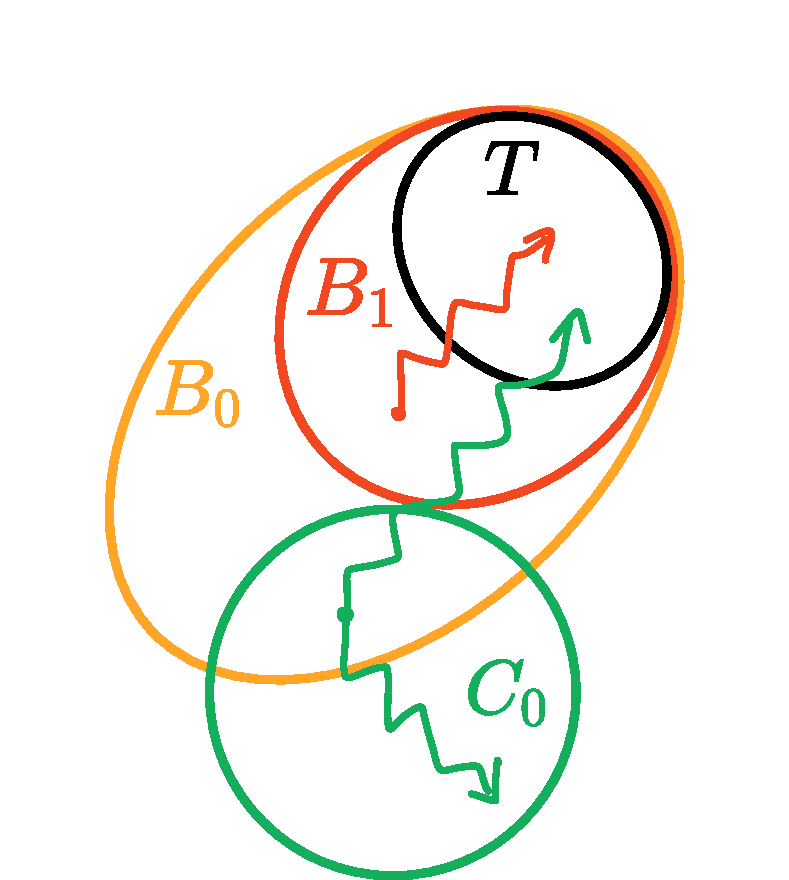
\includegraphics[width=\textwidth]{figures/watr_illustration.pdf}
\end{columns}
    
\end{frame}

\begin{frame}[fragile]{Weak Attractors -- Example\hfill $\watr_0(T=\set{s_1}, \mathcal{P})$}
\centering
\begin{tikzpicture}[>=stealth, node distance=2.5cm, every node/.style={font=\small}]
    % Nodes
    \node[draw, minimum size=1cm, shape=rectangle] (S1) {$\textcolor<2,4,6->{myblue}{s_1}$};
    \node[draw, minimum size=1cm, shape=circle, right=of S1] (S2) {$\textcolor<2,4>{myblue}{\textcolor<5>{orange}{s_2}}$};
    \node[draw, minimum size=1cm, shape=rectangle, right=of S2] (S3) {$\textcolor<2>{myblue}{\textcolor<5>{orange}{s_3}}$};
    \node[draw, minimum size=1cm, shape=circle, right=of S3] (S4) {$\textcolor<3,5>{orange}{s_4}$};

    % Self-loops
    \draw[->] (S1) edge[loop above]
        node[above, pos=0.5] {$\textcolor<2,4,6->{myblue}{(s_1, a)}$} 
        coordinate[pos=0.5] (S1loop) (S1);
    \filldraw[black] (S1loop) circle (2pt);

    \draw[->] (S3) edge[loop above]
        node[above, pos=0.5] {$\textcolor<2>{myblue}{\textcolor<5>{orange}{(s_3, a)}}$} 
        coordinate[pos=0.5] (S3loop) (S3);
    \filldraw[black] (S3loop) circle (2pt);

    \draw[->] (S4) edge[loop above]
        node[above, pos=0.5] {$\textcolor<3, 5>{orange}{(s_4, a)}$} 
        coordinate[pos=0.5] (S4loop) (S4);
    \filldraw[black] (S4loop) circle (2pt);

    % Transitions and splits
    \draw[-] (S1) -- node[below] {} ($(S1)!0.5!(S2)$);
    \filldraw[black] ($(S1)!0.5!(S2)$) circle (2pt) 
        node[label={90:$\textcolor<2,4>{myblue}{\textcolor<5>{orange}{(s_1, b)}}$}] {}; % Labeled split point
    \draw[->] ($(S1)!0.5!(S2)$) -- (S2);
    \draw[->] ($(S1)!0.5!(S2)$) .. controls +(0,-1) and +(0,-1) .. node[below] {} (S1);

    \draw[-] (S2) -- node[below] {} ($(S2)!0.5!(S3)$);
    \filldraw[black] ($(S2)!0.5!(S3)$) circle (2pt) 
        node[label={90:$\textcolor<2,4>{myblue}{\textcolor<5>{orange}{(s_2, b)}}$}] {};
    \draw[->] ($(S2)!0.5!(S3)$) -- (S3);
    \draw[->] ($(S2)!0.5!(S3)$) .. controls +(0,-1.25) and +(0,-1.25) .. node[below] {} (S1);

    \draw[-] (S3) -- node[below] {} ($(S3)!0.5!(S4)$);
    \filldraw[black] ($(S3)!0.5!(S4)$) circle (2pt) 
        node[label={90:$\textcolor<2>{myblue}{\textcolor<3,5>{orange}{(s_3, b)}}$}] {};
    \draw[->] ($(S3)!0.5!(S4)$) -- (S4);
    \draw[->] ($(S3)!0.5!(S4)$) .. controls +(0,-1.5) and +(0,-1.5) .. node[below] {} (S1);

    % No transition from S4 to S1
\end{tikzpicture}

\begin{columns}
    \column{0.65\textwidth}
    \uncover<+->{}
    \begin{align*}
    \uncover<+->{B_0 &= \textcolor<.>{myblue}{\{s_1, s_2, s_3, (s_1, a), (s_1, b), (s_2, b), (s_3, a), (s_3, b)\}}}\\
    \uncover<+->{C_0 &= \textcolor<.>{orange}{\{s_4, (s_3, b), (s_4, a)\}}}\\
    \uncover<+->{B_1 &= \textcolor<.>{myblue}{\{s_1, s_2, (s_1, a), (s_1, b), (s_2, b)\}}}\\
    \uncover<+->{C_1 &= \textcolor<.>{orange}{\{s_2, s_3, s_4, (s_1, b), (s_2, b), (s_3, a), (s_3, b), (s_4, a)\}}}\\
    \uncover<+->{B_2 &= \textcolor<.->{myblue}{\{s_1, (s_1, a)\}}}\uncover<+->{=\watr_0(\set{s_1}, \mathcal{P})}
    \end{align*}
    \column{0.35\textwidth}
    \begin{align*}
        B_0 &\defeq\satr_i(T, \mathcal{P})\\
        C_k &\defeq\satr_{1-i}(S\setminus B_k, \mathcal{P}\setminus T)\\
        B_{k+1} &\defeq\satr_i(T, \mathcal{P}\setminus C_k)\\
    \end{align*}
\end{columns}
\end{frame}



\begin{frame}{Weak Attractors Compute Almost-Sure Reachability}
Let $\mathcal{G}$ be an SMG and $\mathcal{P}$ the corresponding RGN, $i\in\set{0,1}$. It holds that:
\vspace{1cm}

\LARGE
\[
        \watr_i(T, \mathcal{P})\cap S = \ASReach_i(T, \mathcal{G})
\]
\normalsize
\vspace{1cm}

Proof in thesis.
\end{frame}